\begin{question}[index=17,points=10]
设
\[
g(x)=\begin{cases}
f'(0),&x=0,\\[2pt]
\dfrac{f(x)}x,&x\ne0.
\end{cases}
\]
证明：
\begin{enumerate}[label=（\arabic*）,leftmargin=2.5em,labelsep=.4em,itemsep=3pt,topsep=3pt]
\item 若 $f(0)=0$，$f''(0)$ 存在，则有 $\displaystyle g'(0)=\frac12f''(0)$；
\item 若 $f(0)=0$，且 $f(x)$ 在 $(-\infty,+\infty)$ 上有连续的二阶导数，则 $g'(x)$ 在 $(-\infty,+\infty)$ 上连续。
\end{enumerate}
\end{question}
\QuestionBreak\WorkSpace

\begin{question}[index=18,points=12]
设平面光滑曲线 $L$ 位于 $x$ 轴上方并经过点 $M(1,2)$，并且具有如下性质：
从原点到此曲线上任意一点的法线的距离等于该点到 $x$ 轴的距离。
求此曲线方程，并求该方程确定的函数 $y=y(x)$ 的极值。
\end{question}
\QuestionBreak\WorkSpace\WorkPageBreak

\begin{question}[index=19,points=12]
已知 $f(x)$ 是周期为 $2\pi$ 的函数，其在 $[-\pi,\pi]$ 上的表达式为
\[
f(x)=\begin{cases}
x+2\pi,&-\pi\le x<0,\\
0,&x=0,\\
x,&0<x\le\pi,
\end{cases}
\]
将 $f(x)$ 展开为傅里叶级数。
\end{question}
\QuestionBreak\WorkSpace

\begin{question}[index=20,points=12]
计算 $\displaystyle I=\oint_L(y^2-z^2)\dd x+(2z^2-x^2)\dd y+(3x^2-y^2)\dd z$，
其中 $L$ 是平面 $x+y+z=2$ 与柱面 $|x|+|y|=1$ 的交线，
从 $z$ 轴正向看去 $L$ 为逆时针方向。
\end{question}
\QuestionBreak\WorkSpace\WorkPageBreak

\begin{question}[index=21,points=12]
某高速公路网络的交通流量如图所示，其中 $a,b$ 为常数，已知结点 $A,B,C,D$ 处均满足流入量等于流出量，
且该交通网络的流量 $(x_1,x_2,x_3,x_4,x_5)$ 有解。
\begin{enumerate}[label=（\arabic*）,leftmargin=2.5em,labelsep=.4em,itemsep=3pt,topsep=3pt]
\item 求流量通解；
\item 当 $x_4$ 交通封闭时，求此时 $x_2$ 的最大流量。
\end{enumerate}
\begin{center}
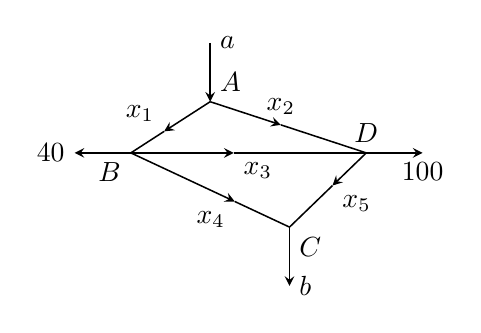
\begin{tikzpicture}[x=.65cm,y=.65cm,line width=.55pt,>=stealth]
  \coordinate (A) at (0,1);
  \coordinate (B) at (-1.55,0);
  \coordinate (D) at (3.05,0);
  \coordinate (C) at (1.55,-1.45);
  \draw[->] (0,2.15) node[right] {$a$} -- (A) node[above right] {$A$};
  \draw[->] (B) node[below left] {$B$} -- (-2.65,0) node[left] {$40$};
  \draw[->] (D) node[above] {$D$} -- (4.15,0) node[below] {$100$};
  \draw[->] (C) node[below right] {$C$} -- (1.55,-2.6) node[right] {$b$};
  \draw[->] (A)--(-.9,.42) node[above left] {$x_1$};
  \draw (-.9,.42)--(B);
  \draw[->] (A)--(1.38,.548) node[above] {$x_2$};
  \draw (1.38,.548)--(D);
  \draw[->] (B)--(.46,0) node[below right] {$x_3$};
  \draw (.46,0)--(D);
  \draw[->] (B)--(.48,-.9495) node[below left] {$x_4$};
  \draw (.48,-.9495)--(C);
  \draw[->] (D)--(2.39,-.638) node[below right] {$x_5$};
  \draw (2.39,-.638)--(C);
\end{tikzpicture}
\end{center}
\end{question}
\QuestionBreak\WorkSpace

\begin{question}[index=22,points=12]
一给水设备每次供水时间为 $2$ 小时，已知该设备启动时发生故障的概率为 $p$。
一旦设备启动，它的无故障工作时间 $X$ 服从指数分布，平均无故障工作时间（$EX$）为 $10$ 小时。
试求设备每次启动无故障工作时间 $Y$ 的分布函数 $F_Y(y)$。
\end{question}
\WorkSpace
